% !TeX root = RJwrapper.tex
\title{GCalignR. An R package for aligning Gas-Chromatography data}
\author{by Meinolf Ottensmann, Martin A. Stoffel, Joseph I. Hoffman}

\maketitle

\abstract{%
Chemical signals are among the most fundamental and oldest means of
animal communication. The desire to unravel broader patterns of chemical
communication in birds and mammals paved the way for two not entirely
new techniques, gas-chromatography and mass-spectrometry, in the fields
of ecology and evolution. Comparing chemical profiles or chromatograms
across many individuals yields some major obstacles as even the newest
GC machines have an inherent error when measuring the retention times of
chemical substances. Here we present GCalignR, an R package for the
alignment of chromatography peaks among samples prior to hypothesis
testing using multivariate statistics. GCalignR is specifically designed
to be used by non-chemists by providing easy to use functions to check
and align gas-chromatography data based on retention times. In addition,
the package implements heatmaps and other plots to evaluate and
potentially adjust the peak alignment. We hope that GCalignR will
provide a tool that fits into a common biologist's workflow in R and
that the package will facilitate the standardization and reproducibility
of studies on chemical communication.
}

\subsection{Introduction}\label{introduction}

Chemical cues are arguably the most common mode of communication among
animals \citep{Wyatt.2014}. Patterns in complex chemical signatures can
can yield information about kinship \citep{Krause.2012, Stoffel.2015},
genetic diversity \citep{Charpentier.2010, Leclaire.2012}, sexual
maturation \citep{Caspers.2011} or be used for species discrimination
\citep{Meulemeester.2011}. One of the most common instruments to
quantify the chemical composition of samples is gas-chromatography (GC),
a fast high-throughput method to detect individual chemicals and their
abundancies \citep{McNair.2011}, while the additional implementation of
mass-spectrometry (GC-MS) allows to identify specific substances
\citep{Caspers.2011}. \par
However, before similarity patterns across samples can be analysed, it
is essential to align compounds. The alignment of samples has to account
for drifts in the retention times of peaks which are caused by subtle,
random and often unavoidable variations of the chromatography machine
parameters \citep{Pierce.2005}. Surprisingly, studies on mammalian or
avian chemical communication often rely on manual alignment rather than
(semi-)automated algorithms, but this approach bears three severe
drawbacks: (1) For larger sample sizes, this task becomes extremely time
consuming and inefficient (2) The researcher may bias the alignment due
to subjective experience and expectations. (3) The data analytical
pipeline from the raw gas-chromatography data to the results of the
statistical analysis is not reproducible. (citations for the first two
points necessary) Several alignment algorithms have been proposed to
overcome these issues, but these focus nearly exclusively on GC-MS data
\citep{Pierce.2005, Robinson.2007,Jiang.2013} and only some are easily
accessible as web-based tools \citep{Hoffmann.2009, Wang.2010} or
independent software \citep{Dellicour.2013}. \par
Here, we introduce \texttt{GCalignR}, an R package that implements a
simple algorithm to align peaks purely from retention time data obtained
by GC and provides sophisticated visualisations for the evaluation of
the alignment quality. \texttt{GCalignR} was specifically developed as a
tool for pre-processing GC data from animal skin and preen glands prior
to subsequent statistical analysis. In brief, the algorithm consists of
two main steps: (1) Systematic shifts of chromatograms are corrected by
applying appropriate linear shifts to whole chromatograms based on a
single reference. (2) Retention times of individual peaks are grouped
iteratively together with homologous peaks of other samples and aligned
within the same row in a retention time matrix . The quality of this
grouping procedure can be adjusted to specific datasets through three
parameters that are described in detail below. Among several optional
processing steps, the package allows to remove peaks that represent
contaminations, which are identified due to their presence in negative
control samples, henceforth called blanks. For an easy interpretation of
the quality of an alignment we implemented several diagnostic plots that
allow to access the aligned data visually. Furthermore, we demonstrate a
complete workflow from chemical raw data to multivariate analyses with
the popular and widely used
\href{https://cran.r-project.org/web/packages/vegan/index.html}{\CRANpkg{vegan}}
\citep{Oksanen.2016} package. This allows the integration of the full
analysis into \strong{RMarkdown} documents \citep{Allaire.2016} in order
to meet the standards of reproducibility \citep{Peng.2011}.

\subsection{The Package}\label{the-package}

\texttt{GCalignR} contains functions to align peaks from GC and GC-MS
data based on retention times and evaluate the respective alignments.
The main aim of the package is to provide a simple tool that guides the
user through the alignment of large data sets prior to the statistical
analysis of multivariate chemical data. An easy workflow for the
analysis of chemical data including \texttt{GCalignR} is shown in figure
\ref{figure:workflow} and described below. The package vignette provides
a detailed description of all functions and their arguments and can be
assessed via \code{browseVignettes('GCalignR')} once the package was
installed.

\begin{figure}[htbp]
  \centering
  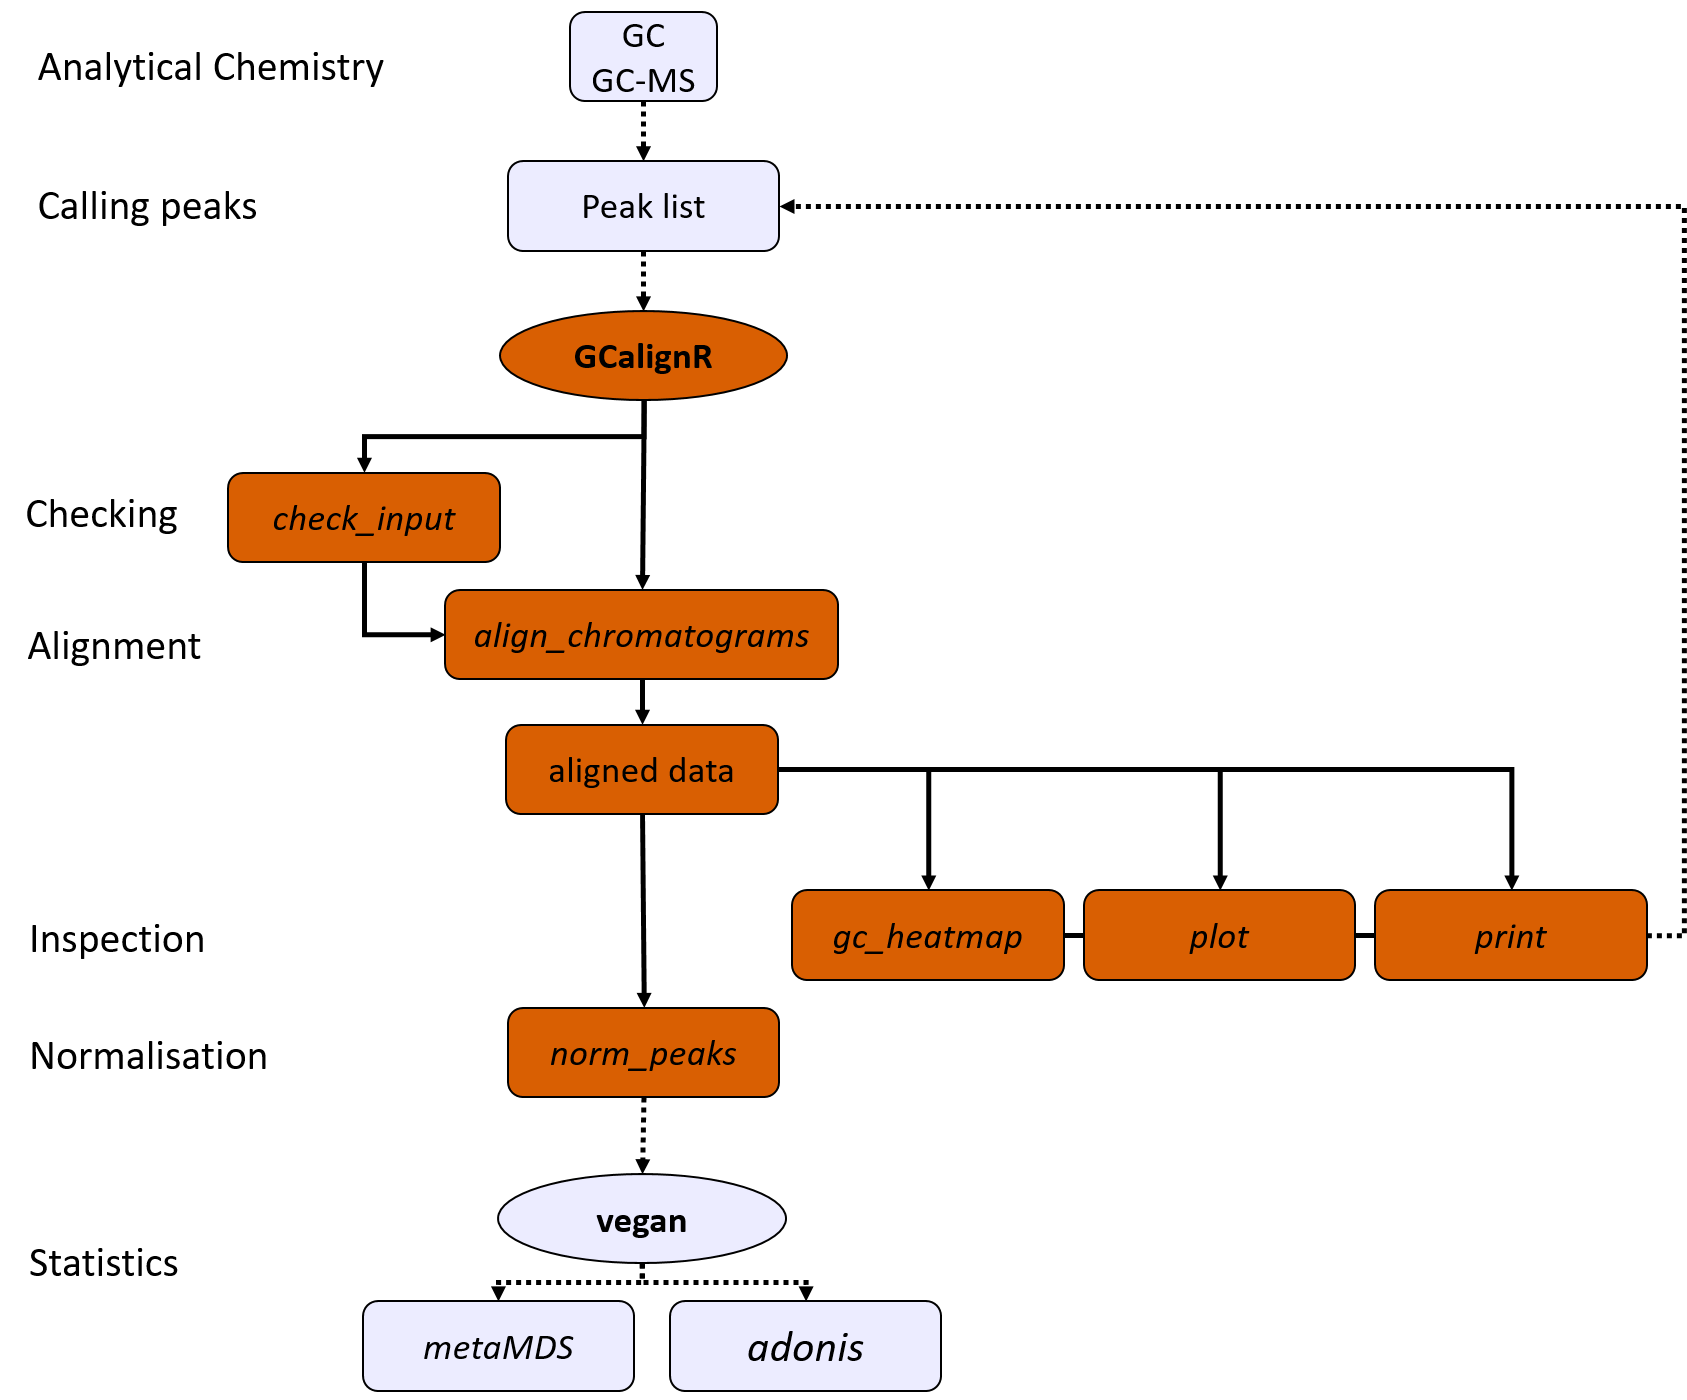
\includegraphics[width=13cm]{figures/workflow}
  \caption{\pkg{GCalignR} workflow. In addition to the alignment of substances across samples, the package provides functions for checking and inspecting the data. The aligned data is ready to use for analyses in conjunction with other packages. Each function is explained within the text.}
  \label{figure:workflow}
\end{figure}

\paragraph{Example dataset}\label{example-dataset}

For demonstration purposes \texttt{GCalignR} includes data of skin
chemicals from 82 Antarctic fur seals \textit{Arctocephalus gazella}. It
was previously shown that these signatures encode the membership to a
breeding colony \cite{Stoffel.2015}. These data are available in a
single text file, the standard input format of \texttt{GCalignR}, that
is distributed with the package. The first two lines contain the names
of all samples and variables respectively. From the third row onwards,
data of all samples is included, whereby data frames are concatenated
horizontally.

\begin{Schunk}
\begin{Sinput}
## Path to the dataset
fpath <- system.file("extdata", "peak_data.txt", package = "GCalignR")
\end{Sinput}
\end{Schunk}\begin{Schunk}
\begin{Sinput}
# Open the file in an external editor
system.file("extdata", "peak_data.txt", package = "GCalignR")
\end{Sinput}
\end{Schunk}

\subsubsection{Alignment of Gas-Chromatography peaks among
samples}\label{alignment-of-gas-chromatography-peaks-among-samples}

The alignment procedure is divided into five steps (figure
\ref{figure:algorithm}). All steps are executed within the main function
\texttt{align\_chromatograms} and will be explained in in the next
sections.

\paragraph{(1) Linear adjustments of
chromatograms}\label{linear-adjustments-of-chromatograms}

At first, all peaks within a chromatogram are shifted with respect to a
reference chromatogram to account for systematic shifts in retention
times among homologous chemicals shared by samples (figure
\ref{figure:algorithm} A). This is done for all samples in relation to
the reference sample such that the number shared peaks is maximised.The
parameter \emph{max\_linear\_shift} defines the maximum temporal range
of linear shifts that are considered by the program. \newline
Note: This method relies on the occurrence of substances that are shared
among most substances to produce efficient adjustments. If those are
absent, it is unlikely to find a suitable shift and chromatograms remain
untransformed. \par
A reference is selected automatically by searching for the sample with
the highest average similarity to all other samples based on the number
of shared peaks prior to alignment. Alternatively, a chromatogram can be
included that contains peaks of an internal standard which peaks are
\textit{a-priori} known to occur in all samples. In this case, the
sample is named \texttt{reference} and will be removed after the
alignment was conducted.

\newpage

\begin{figure}[htbp]
  \centering
  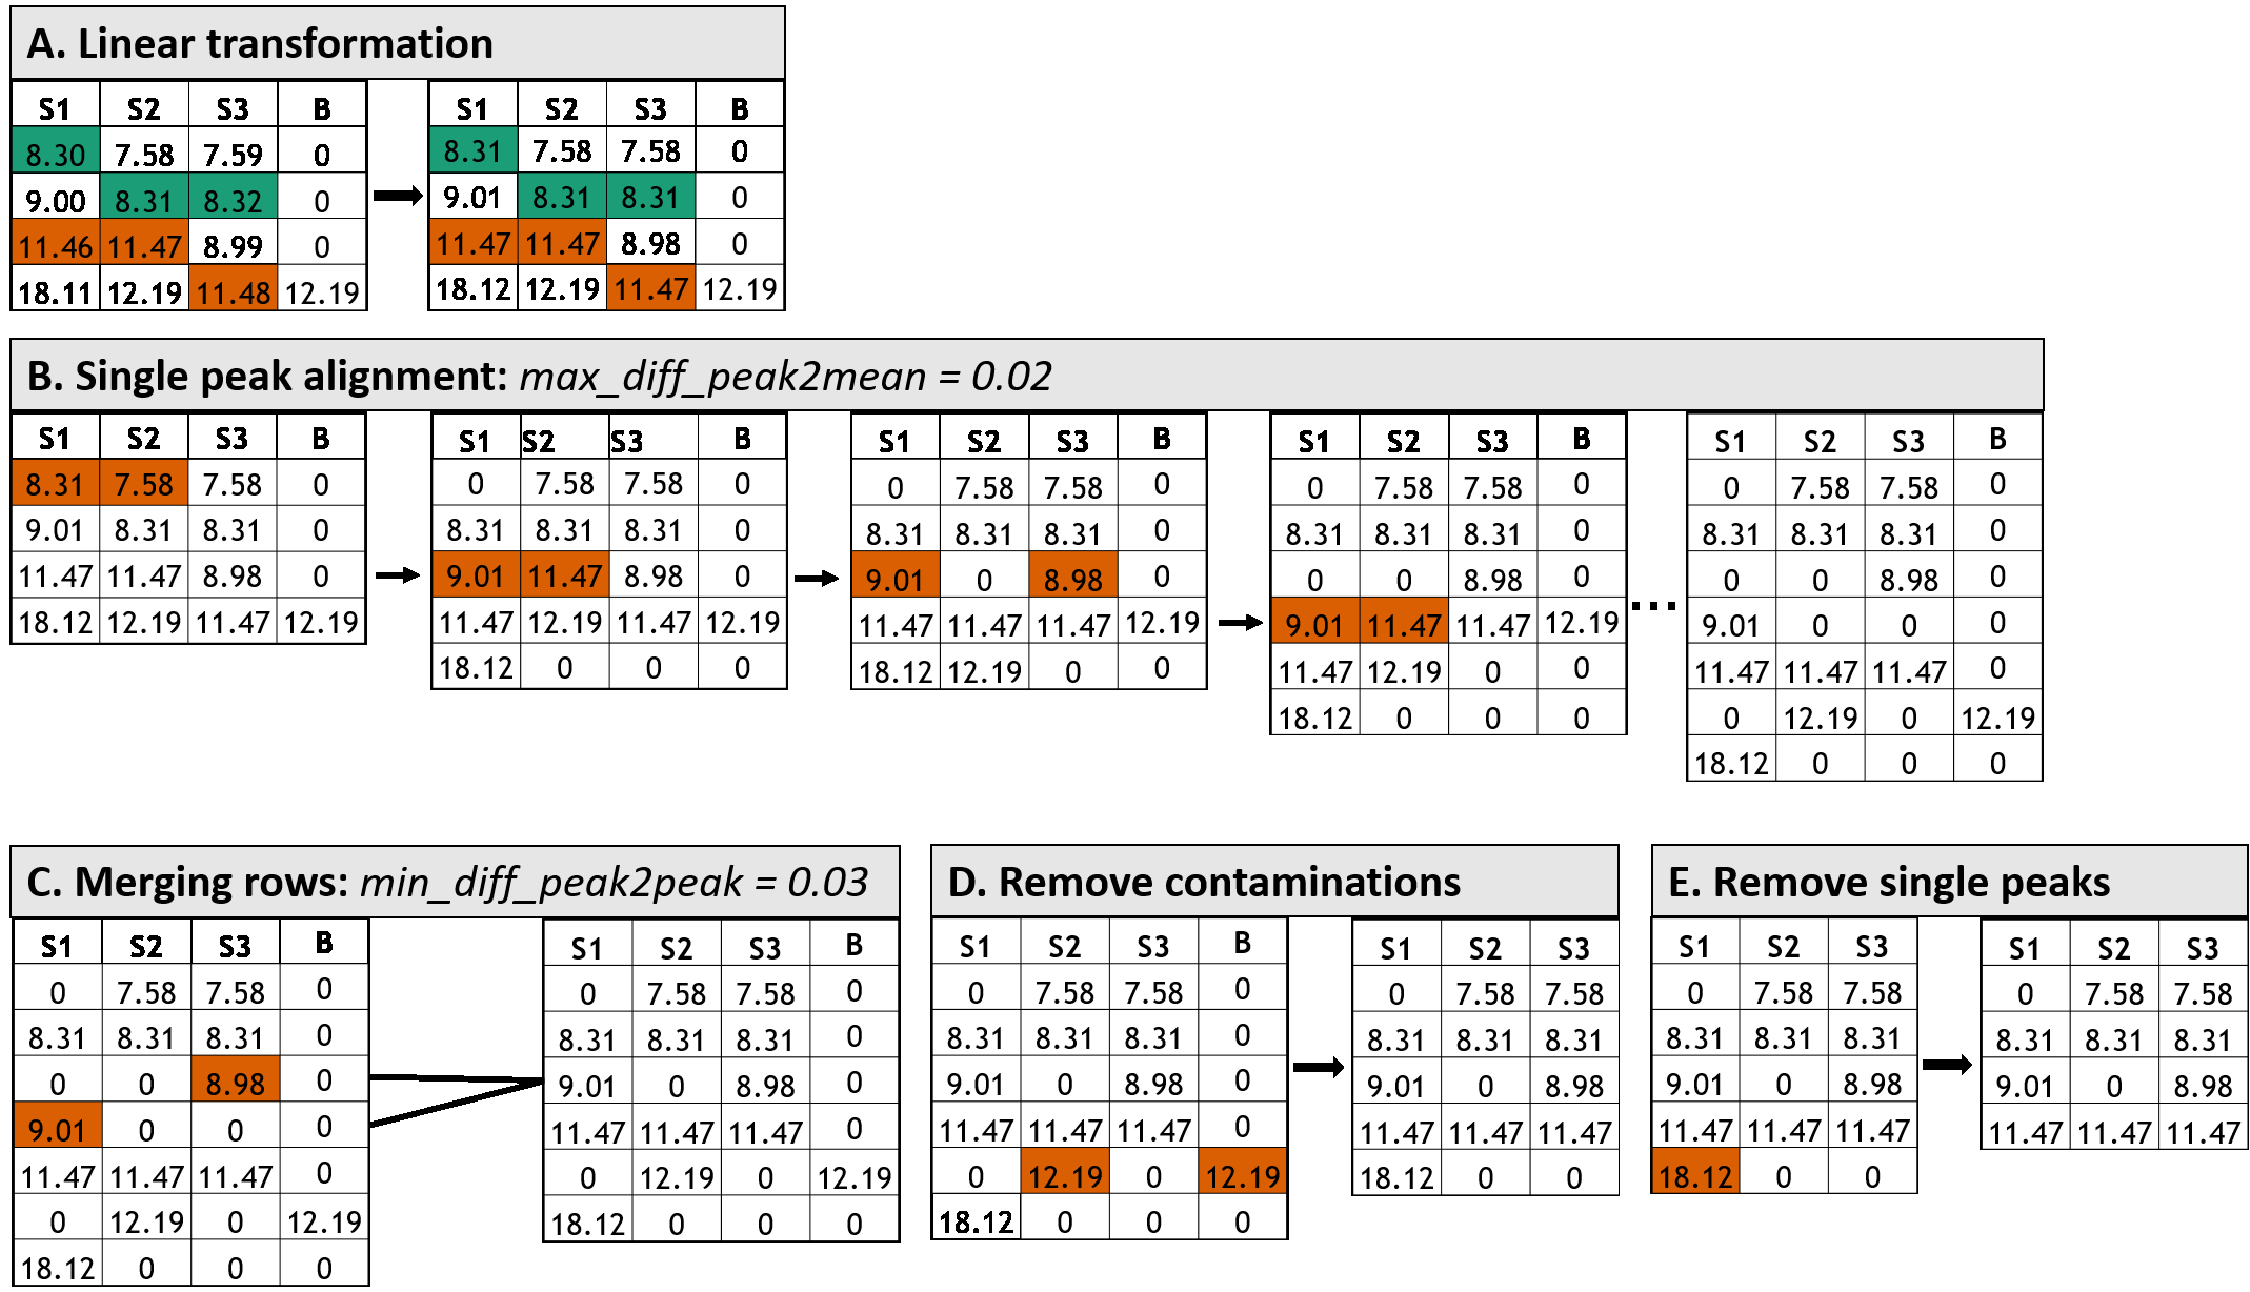
\includegraphics[width=13cm]{figures/algorithm}
  \caption{Overview of the algorithm performed by GCalignR. Rows of matrices correspond to substances, columns are samples. Zeros indicate absence of peaks and are ignored in calculations. \textbf{1}. Chromatograms are linearly shifted with respect to a reference (S2). \textbf{2}. From left to right the first four steps from the input matrix to the final alignment are shown. Peaks are aligned row by row. Initially, always the second sample is compared to the first. Then the next sample is compared to all samples in previous columns until the last column is reached. \textbf{3}. Coloured cells represent conflicting retention times using a minumum \code{max_diff_peak2mean = 0.02}, which defines the minimum difference expected between two distinct substances. If merging does not result in the loss of any data, rows are merged. \textbf{4}. If specified, all peaks found in one or more blanks (negative controls) are removed as well as the blank itself. Unique peaks present in only a single individual are not of interest for similarity analyses and can be removed as well.}
  \label{figure:algorithm}
\end{figure}

\paragraph{(2) Peak alignment}\label{peak-alignment}

The core of the alignment procedure is based on clustering of individual
peaks across samples. This is performed by examining retention times
within single rows, where samples are compared consecutively with all
previous samples starting with the second column (figure
\ref{figure:algorithm} B):\par

\begin{equation}
rt_{m} > \left(\frac{\sum_{i=1}^{m-1}rt_{i}}{m-1}\right) + max\textunderscore peak2mean
\end{equation}

If the examined peak is moved into the next row, whereas all previous
samples are moved \par

\begin{equation}
rt_{m} < \left(\frac{\sum_{i=1}^{m-1}rt_{i}}{m-1}\right) - max\textunderscore peak2mean
\end{equation}

with \textit{rt} = retention time; \textit{m} = current column and
\textit{max\textunderscore diff\textunderscore peak2mean} defining the
maximal deviation of the mean retention time.

By considering the mean retention time among all previous samples the
algorithm accounts for substance specific variations, such that less
variable retention times are treated more stringent than chemicals
exhibiting higher variability. Once the last retention time of a row was
evaluated the whole procedure is repeated with the next row until the
end of the retention time matrix was reached.

\paragraph{(3) Merging}\label{merging}

Sometimes, a single substance has been split up into two different rows.
However, the emerging pattern is very clear, as part of the samples will
have the substance in a given row, but no substance in the adjacent row
and vice versa for another part of the samples. Knowing this pattern,
rows will be merged when this does not cause any loss of any information
(i.e.~no sample exists that contains substances in both rows).(figure
\ref{figure:algorithm} C). Again, the user can change the threshold for
the minimal difference in the retention time between two mergeable peaks
with \textit{min\textunderscore diff\textunderscore peak2peak}. \par 

\paragraph{(4) Post processing}\label{post-processing}

After aligning peaks the package offers several optional post processing
steps that allow to cleanup the data.

\subparagraph{Removing contaminations}\label{removing-contaminations}

Among other sources, residues of unwanted chemical substances in the gas
chromtography column or within reagents used in the laboratory have the
potential to contaminate chemical samples. To get rid of these
substances it is generally advised to include control samples. Within
\texttt{align\_chromatograms} those controls can be included in the data
set in the same way as a normal sample. By specifying the name of one or
more control samples with the
\texttt{blanks\ =\ c("contr1",\ "contr2"),} all substances present in
the control samples are removed from the dataset.

\subparagraph{Removing single peaks}\label{removing-single-peaks}

Sometimes, substances occur purely in a single sample. For comparative
approaches that calculate similarity matrices these substances are often
not informative and can be removed from the data. \texttt{GCalignR}
allows to do so by setting the \texttt{delete\_single\_peak} argument to
\texttt{TRUE}.

\subparagraph{Normalisation}\label{normalisation}

Many multivariate analysis techniques, like those available in
\pkg{vegan}, require a \texttt{data,frame} of independent variables as
input format. Moreover it is generally advisable to normalise substance
abundances prior to statistical analysis to correct for variations in
the total concentration of samples. This can be done in
\texttt{GCalignR} with the function \texttt{normalise\_peaks} which
calculate relative abundances within each sample.

\subsection{Workflow}\label{workflow}

Here, we demonstrate a typical workflow in \texttt{GCalignR} using our
seal data. All alignment steps that have been described above are
implemented within the function \textbf{align\_chromatograms}. A list of
all parameters and their description can be assessed from the
documentation in the helpfile by typing \code{?align_chromatograms}. As
it is outlined in figure \ref{figure:workflow}, the package provides the
function \textbf{check\_input} to test the input file for typical
formatting errors and incomplete data. We encourage to use unique names
for samples that consist only of letters, numbers and underscores. If
the data fails the test, indicative warnings are returned which guide in
correcting those errors. This function ist executed internally prior to
any alignment.

\begin{Schunk}
\begin{Sinput}
check_input(fpath)
\end{Sinput}
\begin{Soutput}
#> All checks passed!
#> Ready for processing with align_chromatograms
\end{Soutput}
\end{Schunk}

\begin{Schunk}
\begin{Sinput}
aligned_peak_data <- align_chromatograms(data = peak_data,
                conc_col_name = "area",
                rt_col_name = "time",
                max_diff_peak2mean = 0.02,
                min_diff_peak2peak = 0.08,
                max_linear_shift = 0.05,
                delete_single_peak = TRUE,
                blanks = c("C2","C3")) # negativ controls
\end{Sinput}
\end{Schunk}

Now, we can inspect the results by retrieving summaries of the alignment
process. The printing method summarises the function call including
defaults that have not been explicitly specified during the function
call. We also get the relevant information to retrace every step in the
alignment:

\begin{Schunk}
\begin{Sinput}
print(aligned_peak_data)
\end{Sinput}
\begin{Soutput}
#>   Summary of Peak Alignment running align_chromatograms from package GCalignR
#>   Input: peak_data   Start:  2017-01-20 17:08:37     Finished:  2017-01-20 17:45:43 
#> 
#> Call:
#>   GCalignR::align_chromatograms(data=peak_data, conc_col_name=area,
#>   rt_col_name=time, max_linear_shift=0.05, max_diff_peak2mean=0.02,
#>   min_diff_peak2peak=0.08, blanks=(C2, C3), delete_single_peak=T, sep=\t,
#>   rt_cutoff_low=NULL, rt_cutoff_high=NULL, reference=NULL)
#> 
#> Summary of scored substances:
#> 
#>     Peaks In_Blanks  Singular  Retained 
#>       497       168        46       283 
#> 
#>   In total 497 substances were identified among all samples. NA substances were
#>   present in blanks. The corresponding peaks as well as the blanks were removed
#>   from the data set. 46 substances were present in just one single sample and were
#>   removed. 283 substances are retained after all filtering steps.
#> 
#> Sample Overview  The following 84 Samples were aligned to the reference 'P31':
#>   M2, M3, M4, M5, M6, M7, M8, M9, M10, M12, M14, M15, M16, M17, M18, M19, M20,
#>   M21, M23, M24, M25, M26, M27, M28, M29, M30, M31, M33, M35, M36, M37, M38, M39,
#>   M40, M41, M43, M44, M45, M46, M47, M48, P2, P3, P4, P5, P6, P7, P8, P9, P10,
#>   P12, P14, P15, P16, P17, P18, P19, P20, P21, P23, P24, P25, P26, P27, P28, P29,
#>   P30, P31, P33, P35, P36, P37, P38, P39, P40, P41, P43, P44, P45, P46, P47, P48
#> 
#> For further details:
#>   Type 'gc_heatmap(aligned_peak_data)' to retrieve a heatmap for the alignment
#>   accuracy
#>   Type 'plot(aligned_peak_data)' to retrieve further diagnostic plots
\end{Soutput}
\end{Schunk}

The quality of an alignment will depend on sensible parameters that
facilitate the (i) correction of linear shifts that might fall in a
larger range with increasing sample size and (ii) and the variability of
retention times. Optimally, linear shifts do not exhaust the range given
by \texttt{max\_linear\_shift} completely, which would in turn indicate
that not all uncertainties haven been fully compensated for. This can be
assessed by four diagnostic plots that can be created alltogether as
well as individually.

\begin{Schunk}
\begin{Sinput}
plot(aligned_peak_data)
\end{Sinput}

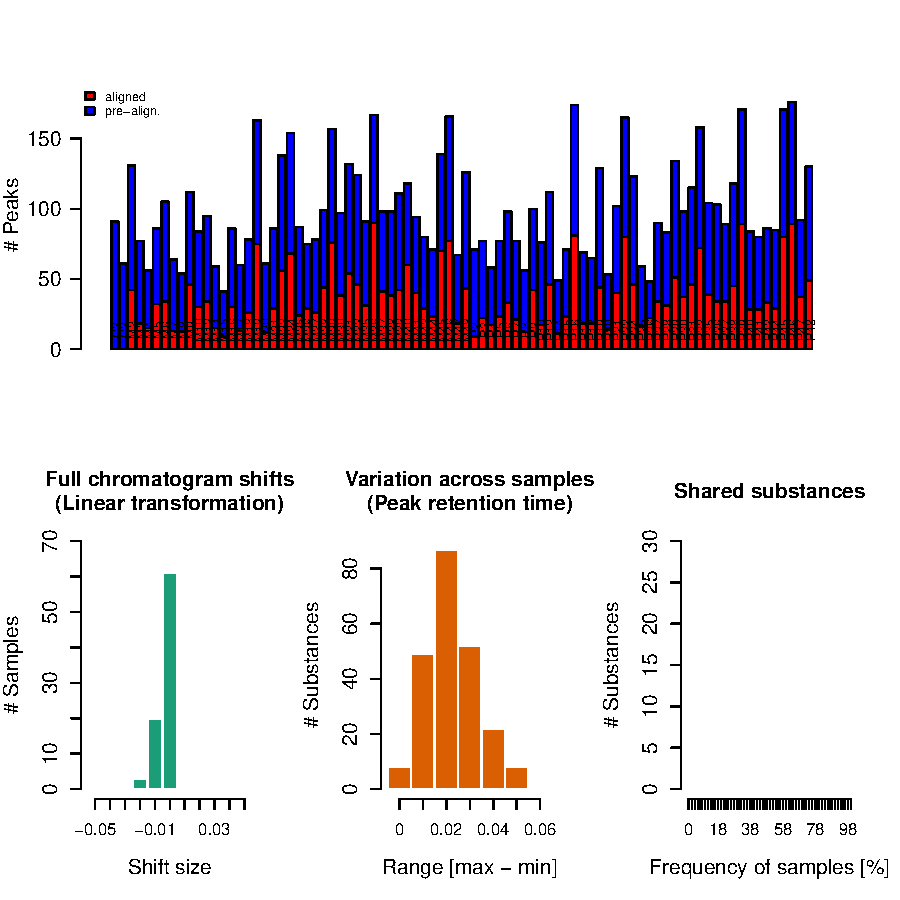
\includegraphics{ottensmann-stoffel-hoffman_files/figure-latex/unnamed-chunk-7-1} \end{Schunk}

The distribution of peak number before and after the alignment reveals a
noticeable reduction of peaks in the aligned dataset. These changes can
be explained by the removal of contamimations (i.e.~peaks present in
blanks) and the removal of single peaks. Type
\code{print(aligned_peak_data)} for details on both. The distribution of
shifts size used for linear transformations shows a marginal linear
trend across the chromatography run. Besides the pure number of peaks it
is of major interest to inspect the distribution of substances in the
pool of samples and access the variation in retention times. This can be
investigated simultaneously with a heatmap.

\begin{Schunk}
\begin{Sinput}
gc_heatmap(aligned_peak_data,type = "discrete", substance_subset = 1:25, samples_subset = 1:25)
\end{Sinput}

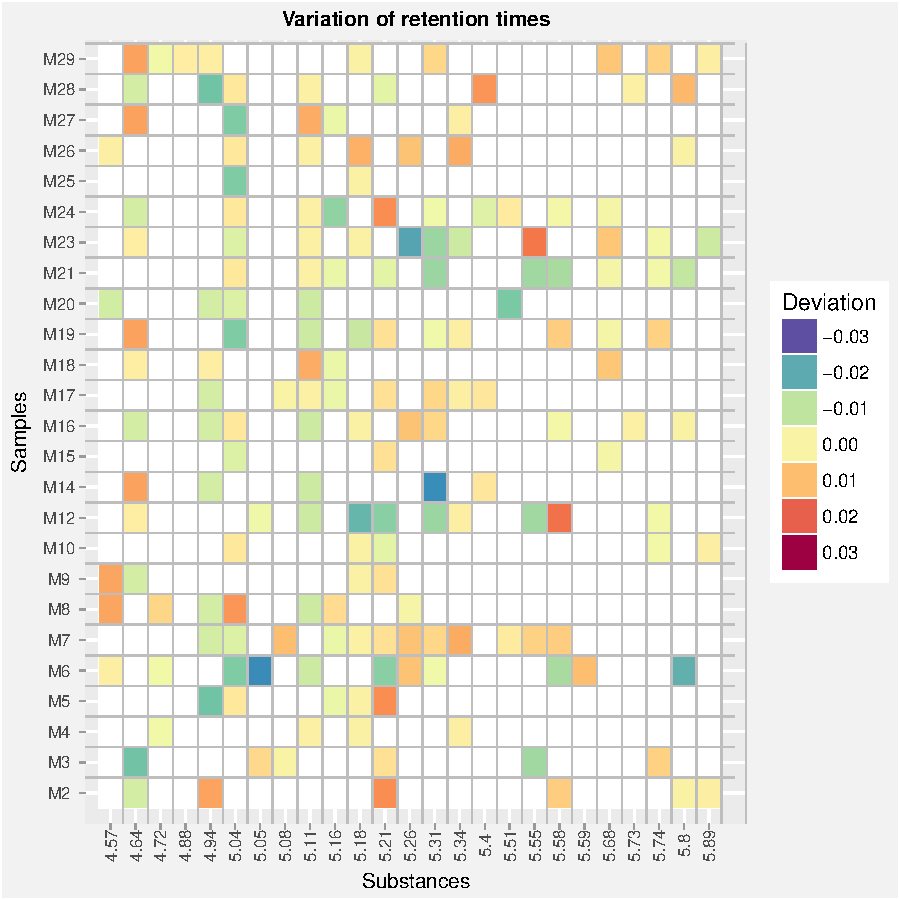
\includegraphics{ottensmann-stoffel-hoffman_files/figure-latex/unnamed-chunk-8-1} \end{Schunk}

The heatmap indicates the presence of a certain substance within a
sample by a colour-filled box, whereas the absense is encoded by a white
box. Furthermore a colour-gradient is used to indicate the deviation of
each retention time from the mean value among all other samples as a
measure of variation. \bibliography{ottensmann-stoffel-hoffman}

\address{%
Meinolf Ottensmann\\
Department of Animal Behaviour\\
Bielefeld University\\ Morgenbreede 45\\ 33615 Bielefeld\\
}
\href{mailto:Meinolf.Ottensmann@web.de}{\nolinkurl{Meinolf.Ottensmann@web.de}}

\address{%
Martin A. Stoffel\\
Department of Animal Behaviour\\
Bielefeld University\\ Morgenbreede 45\\ 33615 Bielefeld\\
}
\href{mailto:Martin.Adam.Stoffel@gmail.com}{\nolinkurl{Martin.Adam.Stoffel@gmail.com}}

\address{%
Joseph I. Hoffman\\
Department of Animal Behaviour\\
Bielefeld University\\ Morgenbreede 45\\ 33615 Bielefeld\\
}
\href{mailto:j_i_hoffman@hotmail.com}{\nolinkurl{j\_i\_hoffman@hotmail.com}}

